\documentclass[10pt,a4paper]{article}
\usepackage[latin1]{inputenc}
\usepackage[english]{babel}
\usepackage{amsmath}
\usepackage{amsfonts}
\usepackage{amssymb}
\usepackage{graphicx}
\usepackage{fancyhdr}
\usepackage{lastpage}
\usepackage{multirow}

%Include and define  c code
\usepackage{listings}
\usepackage{color}
\usepackage{textcomp}
\definecolor{listinggray}{gray}{0.9}
\definecolor{lbcolor}{rgb}{0.9,0.9,0.9}
\lstset{
	language=C,
	keywordstyle=\bfseries\ttfamily\color[rgb]{0,0,1},
	identifierstyle=\ttfamily,
	commentstyle=\color[rgb]{0.133,0.545,0.133},
	stringstyle=\ttfamily\color[rgb]{0.627,0.126,0.941},
	showstringspaces=false,
	basicstyle=\small,
	numberstyle=\footnotesize,
	numbers=left,
	stepnumber=1,
	numbersep=10pt,
	tabsize=2,
	breaklines=true,
	prebreak = \raisebox{0ex}[0ex][0ex]{\ensuremath{\hookleftarrow}},
	breakatwhitespace=false,
	aboveskip={1.5\baselineskip},
  columns=fixed,
  upquote=true,
  extendedchars=true,
 frame=single,
 backgroundcolor=\color{lbcolor},
}

\oddsidemargin  -0.5cm
\evensidemargin 0.0cm
\textwidth      17.25cm
\headheight     1.0cm
\headsep		0.7cm
\topmargin      -0.5cm
\textheight		22.0cm

\pagestyle{fancy}
\lhead{Exercise 5}
\chead{EEMB1}
\rhead{\thepage\ of \pageref{LastPage}}
\lfoot{Theis Christensen\\Paulo Fontes\\Dennis Madsen}
\cfoot{Team3}
\rfoot{\today}
\renewcommand{\headrulewidth}{0.4pt}
\renewcommand{\footrulewidth}{0.4pt}
\begin{document}
\part*{EMB 2010 Team3 ExerciseADC}

\section{R2R ladders}
http://en.wikipedia.org/wiki/Resistor\_ladder
\begin{figure}[htbp!]		%Remember to put the h!, to not fuck the sections.
	\begin{centering}
 		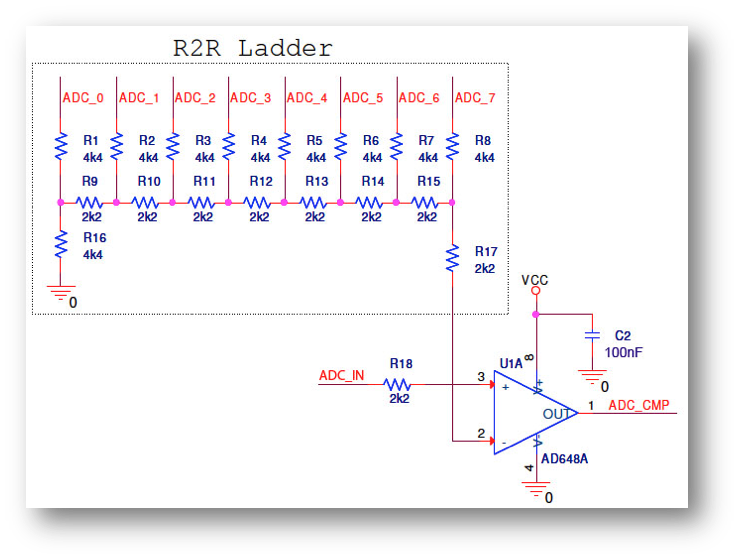
\includegraphics[width=1.0\textwidth]{images/r2r.png}
		\caption{r2r ladder}
	\end{centering}
\end{figure}
\newpage
\section{Successive Approximation technique (SAR)}
The successive approximation technique uses an comparator to check for comparison between the voltage that wants to be read and an internal
value that represents the middle value of the current range.
\\ \textbf{Example VREF = 5}
\begin{itemize}
	\item Internal value set to half the range 5 - 0 = 2.5V
	\item Value is \textbf{below}, new range 2.5 - 0 = 1.25V
	\item Value is \textbf{above}, new range 2.5 - 1.25 = 1.875
	\item Value is \textbf{below}, new range 1.875 - 1.25 = 1.5625
	\item Value is \textbf{above}, final value = \textbf{1.875}
\end{itemize}
\begin{figure}[h!]		%Remember to put the h!, to not fuck the sections.
	\begin{centering}
 		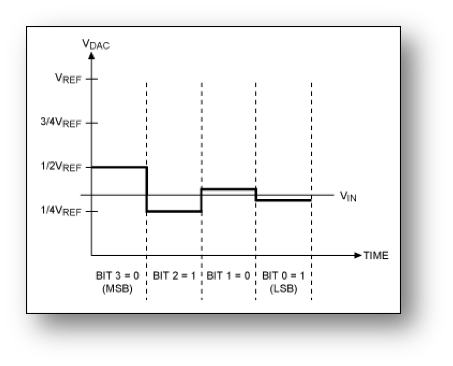
\includegraphics[width=0.7\textwidth]{images/sar.png}
		\caption{4-bit Successive Approximation Register}
	\end{centering}
\end{figure}
\newpage
\section{Flash conversion technique}
\textbf{Flash conversion / Flash ADC / Direct-Conversion ADC}\\
This setup has a bank of comparators which makes it possible to sample the input signal in parallel, where each comparator have a certain voltage range.
All the comparators feeds an logic circuits which generates a binary code of the inputted voltage.\\
\\ \textit{Note that ADC using this circuit setup is rarely seen in bigger resolutions than 8 bits as the amount of comparators needed doubles for each bit added to the precision.}
\begin{figure}[h!]		%Remember to put the h!, to not fuck the sections.
	\begin{centering}
 		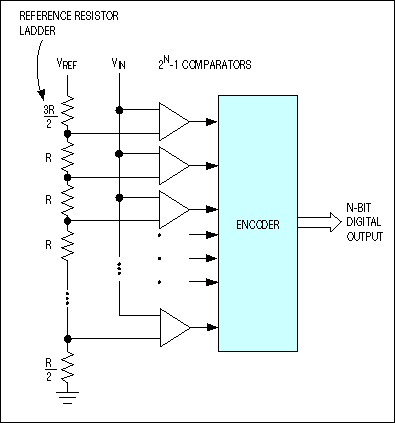
\includegraphics[width=0.6\textwidth]{images/flash_conv.png}
		\caption{Flash conversion setup}
	\end{centering}
\end{figure}
\newpage
\section{Sigma Delta conversion principle}
Down below an example of implementing the Sigma Delta is shown.
\\ The circuit simply counts how many trigger pulses that have occurred within a certain time (specified by the 'Summing Interval') and
from that a frequency is calculated.
\begin{figure}[h!]		%Remember to put the h!, to not fuck the sections.
	\begin{centering}
 		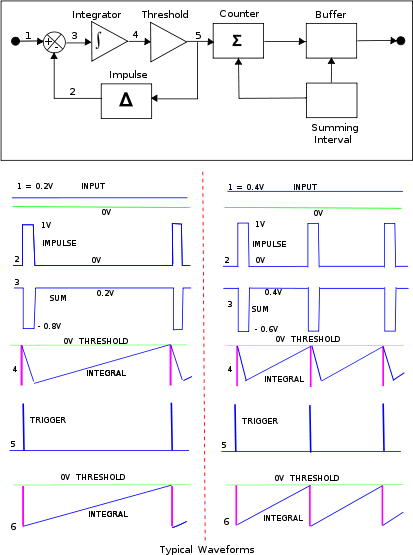
\includegraphics[width=0.7\textwidth]{images/sigma_delta.png}
		\caption{Block diagram of an sigma-delta ADC}
	\end{centering}
\end{figure}

\newpage
\begin{figure}[h!]		%Remember to put the h!, to not fuck the sections.
	\begin{centering}
 		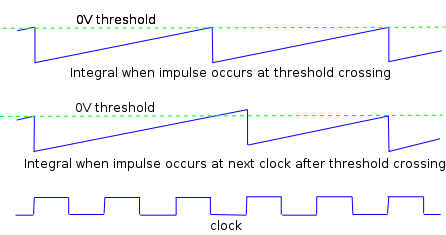
\includegraphics[width=0.6\textwidth]{images/sigma_delta2.png}
		\caption{Block diagram of an sigma-delta ADC}
	\end{centering}
\end{figure}

\newpage
\section{Sample and hold circuits}
The sample and hold circuit is used to 'freeze' the analog value at a time and thereafter read the value.
\begin{figure}[h!]		%Remember to put the h!, to not fuck the sections.
	\begin{centering}
 		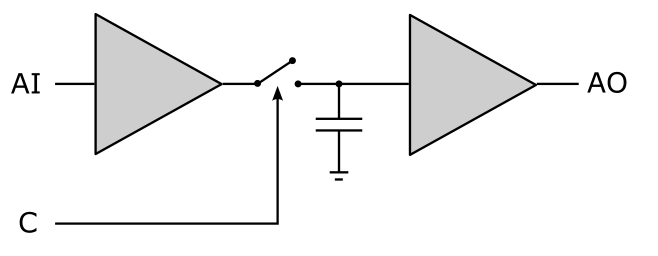
\includegraphics[width=0.5\textwidth]{images/sample_hold.png}
		\caption{Threshold voltage }
	\end{centering}
\end{figure}

\newpage
\section{Bandwidth vs. resolution for the different types}
What conversion type is the fastest, and which one is the most precise?

\end{document}
